\documentclass[a4]{article}
\usepackage{fullpage}
\usepackage{biblatex}
\usepackage{listings}
\usepackage{placeins}
\usepackage{graphicx}
\lstset{captionpos=b}
\bibliography{refs.bib}
\title{Advanced database systems: Homework 6}
\author{Leendert Dommicent and Jorn Van Loock}
\date{}
\begin{document}
\maketitle
\setlength{\parindent}{0px}
\setlength{\parskip}{8px}
\section{Introduction}
This document describes what we have don for the final homework. In section \ref{sec:problem} we will describe the problem domain and why the data mining project that we have carried out can be usefull. In section \ref{sec:gathering_data} we will explain where we got the data from and why we chose these data sources. Next in section \ref{sec:preparing_data} we explain how the data is prepared for use with Weka. Which data do we drop and why, which data we combine and so forth. In section \ref{sec:weka} we will describe how we will use Weka to find interesting results in the data. Section \ref{sec:results} will explain the results that we have and what they imply. Finally in section \ref{sec:conclusion} we will formulate a conclusion about this homework.
\section{The problem domain}
\label{sec:problem}
Almost every day the world suffers under terrorist attacks. Those attacks are carried out by individuals in their own name or in the name of a bigger organisation. New terrorist organizations start when other stop. For these new organizations the whole investigation about their actions must be done all over again. Wouldn't it be great if we could learn from the existing and past organizations and apply this on the newly created organizations? In a very minimal way, this is after all a homework and not a thesis, we will try to do this.\par
All terrorist attacks can be classified by a type, for example bombing or hostage taking. They also target a specific victim type like the government or a private company. We can also classify the different types of terrorist organizations. You have organizations with a cultural background and others with a political.\par
In this research we want to determine if there is a connection between the type of terrorist organization, the continent they are active in and the type of attacks they are doing. Wouldn't it be interesting if a new terrorist organization rises we can predict which attack type they will use or which people they are most likely to attack? We are very confident that this is a very interesting and useful domain to do research in.
\section{Gathering the right data}
\label{sec:gathering_data}
To predict this we first have to acquire the necessary data of the terrorist organizations we know. We need to know the types of organizations, the attacks they do and where they do it.\par
For the attacks we used GTD (Global Terrorist Database)\cite{gtd}. This database contains terrorist attacks all over the world. It contains the countries where they were executed, the type of the attacks and the type of the victims. We wrote a Java parser that parsed all these attacks and added them to an OWL ontology. You can find more information in this\cite{homework2} report.\par To know in which continent the countries of the attacks are located we used the CIA World Factbook\cite{factbook}. We also wrote a Java parser for this database and added the content to our owl ontology. Again you can find more information in this\cite{homework2} report.\par
We also needed more information about the organizations themselves. For this we used the Terrorist Organization Profiles database\cite{start}. This database is from the same makers as GTD so names from the two databases should match. Because of this we do not have double individuals with a slightly different name in our OWL database. So also for this database we wrote a Java parser to add the data to our ontology. More information of this you can find in this\cite{homework3} report.\par
We now have all the data we need in an OWL ontology. This ontology file also has an accompanying readme file. In this file you can find how the ontology itself is build up. Which classes and what sort of individuals it contains. It also explains which relations (object and data) are in the ontology and for which individuals they are filled in. In the next section we will describe how we will transform this data to be able to use Weka.
\section{Preparing the data}
\label{sec:preparing_data}
We need to convert our OWL ontology to an ARFF file that can be read by Weka. On the way we will simplify the data a little bit. We will write this converting program in Java. We need a way to read out our OWL ontology. For this we used the OWLAPI\cite{owlapi}. This is a powerful API for Java that allows you to read and write data to and from your ontology. We already used it to write and populate our ontologies decsribed in the previous section but will now use it to read certain elements from the ontology.\par
We have three different ways that we prepared the data. We will explain them all. The results of the data mining depends on the way we prepared the dataThis means that also the section \ref{sec:results} is devided in three parts, one for every way we prepared the data.\par
\subsection{1 entry for every terrorist organization}
\label{sec:1_for_organization}
To begin the first conversion we will search all attack individuals from our ontology. For every individual we will first get the terrorist organization that is responsible for the attack. If we didn't already came across this organization we will create a new organization object otherwise we will use the existing object. We will then add the country of the attack and his victim type and attack type to this organization object. If any information is missing we will just ignore the current attack. After this step is completed we have an object for every terrorist organization. This object contains all the victim types and attack types they have used, the amount of each of the types and the countries in which they operate. Now we only need the type of organization of the organization. So we search for this information in the OWL ontology and add this to the object. Again when we do not find the type in the ontology we drop the organization, because it just isn't useful for learning.\par
In the next step we have to simplify the data in de objects and write it to an ARFF file. First we are going to simplify the countries of the organization object. For every country in the object we will search the continent of that country. Then we will count which continent is the most occurring and throw away the other continents. We do the same for the attack types and the victim types, so only the most occurring are kept. We do understand that we make a huge generalisation by simplifying the data like this.\par
Now we have to convert all this organization objects to an ARFF file. First we have to create the heading of the ARFF file. To do this we have to identify the attributes of the problem and the instances. The instances are clearly the terrorist organizations. The attributes are the name of the organization, the type of the organization and the most used victim type and attack type. The first attribute is a simple string and isn't used in the actual data mining. It is just used to keep the ARFF file more clear. The other type are nominal. This means that we have to declare all the possible values up front in the header of the file. To do this we retrieve all the possible continents, attack types and victim types and add them to the header of the ARFF file. You can find the resulting header in figure \ref{fig:arff_header}. Notice that all the spaces are replaced by underscores. This is because we noticed that Weka gives errors when there are spaces in the content of attributes. So we replace spaces by underscores in the entire ARFF file. Also the (') sign gave problems so we just deleted them in the entire file.\par
In figure \ref{fig:arff_header} you can see which possible values we use. You can see that we do not just use continents but that we sort of split up the large continents. In total we have 10 possible continent values. We hope that this split up gives us better result instead of just using the normal continents. We also thought about using countries instead of continents, but we are afraid that this gives us results that are too specific and are by consequence not very useful.\par
\begin{figure}[!h]
\centering
\begin{tabular}{c}
\begin{lstlisting}
@Relation titanic
@ATTRIBUTE name string
@ATTRIBUTE classification {Anarchist,Anti-Globalization,Communist/Socialist,
Environmental,Leftist,Nationalist/Separatist,Racist,Religious,
Right-Wing_Conservative,Right-Wing_Reactionary,n/a,Other}
@ATTRIBUTE continent {Africa,Australia-Oceania,Central_America_and_Caribbean,
Central_Asia,East_&_Southeast_Asia,Europe,Middle_East,North_America,
South_America,South_Asia}
@ATTRIBUTE victimType {Abortion_Related,Airports_&_Airlines,Business,
Educational_Institution,Food_or_Water_Supply,Government_(Diplomatic),
Government_(General),Journalists_&_Media,Maritime,Military,NGO,Other,Police,
Private_Citizens_&_Property,Religious_Figures/Institutions,Telecommunication,
Terrorists,Tourists,Transportation,Unknown,Utilities,Violent_Political_Party}
@ATTRIBUTE attackType {Armed_Assault,Assassination,Bombing/Explosion,
Facility/Infrastructure_Attack,Hijacking,Hostage_Taking_(Barricade_Incident),
Hostage_Taking_(Kidnapping),Unarmed_Assault,Unknown}
@DATA
\end{lstlisting}
\end{tabular}
\caption{The header of the created ARFF file}
\label{fig:arff_header}
\end{figure}
\par
Now that we have the header we have to convert every object to an instance and by consequence a line in the ARFF file. You can find the structure of the line in figure \ref{fig:entry}. Notice that they are just the properties of the organisation object separated by a comma.\par
\begin{figure}[!h]
\centering
\begin{tabular}{c}
\begin{lstlisting}
name_organization,type_organization,continent,victim_type,attack_type
\end{lstlisting}
\end{tabular}
\caption{An instance entry in the ARFF file}
\label{fig:entry}
\end{figure}
\subsection{1 entry for every attack}
\label{sec:1_for_attack}
Maybe the simplification of all victim types and attack types from every attack to one for every terrorist organization is too hard. Maybe it's a better solution to give weka this information for every attack. To do this we have to change our precious Java program.\par
The Java program from section \ref{sec:1_for_organization} creates one object for every terrorist organization. If it iterates over an attack of an organization for which the terrorist organization object is already initialized, it will just return this object to work with. It will then for example add another attack type to this object. To make the requested modification we just have to create a new terrorist organization object for every attack in the database. In the rest of this section we will call this object an entry object to keep things clear. So we just remove the code that checks if the entry object is already created. The rest of the code that simplifies the entry objects is now unnecessary but we can leave it there. Because every entry object now has only one victim type and one attack type, because an attack has only one victim type and one attack type, it is automatically selected by the simplification algorithm.\par
The structure of the resulting ARFF file is the same as in section \ref{sec:1_for_organization}. However in section  \ref{sec:1_for_organization} we have a line like the one in figure \ref{fig:entry} for every organization. Now however we have such a line for every attack but with the same structure. So for example if the IRA has carried out multiple attacks they will have multiple entries in the file. So with this way of preperation we have a much bigger file than the first way. In the file of \ref{sec:1_for_organization} we have around 200 entries, with this system we have around 13000 entries. So with this method we have a lot more data to work with.
\subsection{1 entry for every attack with neighbours}
\label{sec:withneighbours}
While we were explaining our plans for this homework, it was brought to our attention that continent is maybe a too general feature. Maybe it was better to work with regions instead of full continents even when we split some big continents up. Because of the time constraints of this project it wasn't feasible to manually enter a region for every country. We also didn't find a good data source that contained this data. So we had to come up with another solution that made us able to split up the continents in smaller pieces and which could be done in an automated fashion.\par
We found a solution that would chain neighbouring  countries together. So for every attack we fetch the country and add it to the entry object. After we do this we traverse all created entry objects. For every object we get the neighbouring countries of the country contained by the object and add it to the object. We then delete duplicate countries. If we want to we can do this 2 steps several times to make the regions bigger. For this homework however we will not do this but the code can be extended easily to support this. We now have entry objects that contain the country of the attack and the neighbouring countries. We now have to translate this to an ARFF file.\par
To translate this we will use the structure you can find in table \ref{fig:structure_arrf_3}. So we kept all the features from the previous methods but we added one for every country in the database. This feature will contain zero or one depending of the fact if the attack took place in this country or in a neighbouring country.\par
\begin{table}[!h]
\centering
\begin{tabular}{|c|c|c|c|c|c|c|c|c|}\hline
Name & Type & Continent & VictimType & AttackType & Afghanistan & Albania & ... & Zimbabwe \\ \hline
\end{tabular}
\caption{Structure of the ARFF file with the third method}
\label{fig:structure_arrf_3}
\end{table}
We now need to expend the functionality of our Java program to fill in the structure. We added a method who created a string for every entry object with comma separated zero's and one's depending on which countries the entry object contains. We then concatenate this string with the old string. You can find the result of an existing entry in table \ref{fig:example_arrf_3}. In the ARFF file this data is of course comma separated like the other methods.\par
\begin{table}[!h]
\centering
\begin{tabular}{|c|c|c|c|c|c|c|c|c|}\hline
Name & Type & Continent & VictimType & AttackType & Afghanistan & Albania & ... & Zimbabwe \\ \hline
JRA & Communist & Asia & Airports & Hijacking & 0 & 1 & ... & 0 \\ \hline
\end{tabular} 
\caption{Example of a fictive entry}
\label{fig:example_arrf_3}
\end{table}
The final thing we have to do is adapt the ARFF header of the previous methods to accommodate the new features. To do this we wrote a method in our Java program that gets all countries inside the ontology. For every country found it will write the line in figure \ref{fig:country_header} to the header of the ARFF file. All this entries make the header much bigger than before. You can see that it is a nominal feature that can contain the values zero and one like previously explained.
\begin{figure}[!h]
\centering
\begin{tabular}{c}
\begin{lstlisting}
@ATTRIBUTE name_country {0,1}
\end{lstlisting}
\end{tabular}
\caption{A country entry within the ARFF header}
\label{fig:country_header}
\end{figure}
To make the whole ARFF file a little bit smaller we deleted all country columns who contained only zero's and adapted the ARFF header accordingly.
\subsection{The resulting Java program}
You can find the resulting program in our GitHub repository\cite{githubproject} which is publicly available. The class \textit{FactbooktoARFF} in package \textit{com.conbit.factbookparser.convertors} handles the actual conversion from OWL to ARFF. It contains booleans to determine which method of the three we explained you want to use.
\section{Using Weka for data mining}
\label{sec:weka}
To be able to predict the attack types and victim types of future terrorist organizations we need to learn some rules about them. We can also try to find a way to classify the current organizations and if a new organization comes up we can classify them and by result know their preferred attack and victim type. Before starting the mining algorithm on the data we first have to remove the feature name because it isn't relevant, it was just there for debugging purposes. This can easily be done in Weka.\par
First we will try to find certain rules in the data. An example of such a rule could be: \textit{Religious organizations that operate in Europe mostly use hostage tacking as their attack type.} For this rule mining we will try to use the rule miner Apriori. Apriori will try to find rules between a certain metric. You can for example state that it has to find rules with a confidence higher then 0.9 for example. We will use Weka with the standard parameters only the minimum confidence is changed to 0.5 to get more result. With these parameters Apriori will try to find rules with a certain support it will then lower the support and try again. He will do this until he has found 10 rules. The minimum support is 0.1 with the default parameters. If we have changed the minimum support for a certain test we will explicitly mention it.\par
Next we will try to classify the different organizations using a decision tree. To build this tree we are planning to use the J48 algorithm of Weka. This algorithm can build such a decision tree. With this tree we can than classify new organizations and identify which attack and or victim types they will try to use. We will run the J48 algorithm again with the standard parameters. We will always build 2 trees, one for prediction the victim type and one for the attack type.\par
\section{Results}
\label{sec:results}
In this section we will give the results from Weka for the three data files, one for each preparing method. We will also try to interpret this message. For every preparing method we will give the results of both Apriori and J48.
\subsection{Results for datafile with 1 entry for every organization}
In this section we will give the results for the datafile constructed in section \ref{sec:1_for_organization}.
\subsubsection{Apriori}
\FloatBarrier
\begin{figure}[!h]
\centering
\begin{tabular}{c}
\begin{lstlisting}
1. victimType=Business 51 ==> attackType=Bombing/Explosion 39    conf:(0.76)
2. continent=Middle_East 41 ==> attackType=Bombing/Explosion 26    conf:(0.63)
3. continent=Europe 67 ==> attackType=Bombing/Explosion 42    conf:(0.63)
4. classification=Other 46 ==> attackType=Bombing/Explosion 28    conf:(0.61)
5. classification=Religious 55 ==> attackType=Bombing/Explosion 31    conf:(0.56)
6. victimType=Business 51 ==> continent=Europe 27    conf:(0.53)
7. classification=Nationalist/Separatist 53 ==> attackType=Bombing/Explosion 28    conf:(0.53)
\end{lstlisting}
\end{tabular}
\caption{Apriori results for first data file}
\label{fig:apriori_1}
\end{figure}
In figure \ref{fig:apriori_1} you can find the result of the Apriori data mining in Weka. At first sight it seems that it generated some interesting rules. However if we look closer we see that it almost always predicts the attack type \textit{Bombing/Explosion}. Rule 5 is interesting because it tells us that most businesses that have been attacked are in Europe. However this rule does not have a large confidence.\par
We changed to minimum support to 0.05 for a second test which we think is pretty low in a dataset of 231 instances. However Weka only generated more rules with a prediction of \textit{Bombing/Explosion} as attack type. So the only information we in fact really got is that most terrorist attacks are bombings.
\subsubsection{J48}
The tree for the attack type only has one leaf \textit{Bombing/Explosion}. The three classifies 55\% correctly according to 10-fold cross-validation. This confirms the rules of Apriori. The most attacks that are being executed are bombing attacks.\par
The tree for the victim types only classified 27\% correctly. It however did have 1 interesting branches. Bombing attacks in Europe mainly focus on business targets, this is true in 22 of the 42 occurrences. This was the branch with the best confidence and a decent support. And still the confidence isn't high. This resulting tree is quite bad, so that maybe explains why Apriori couldn't give any rules.
\subsubsection{Conclusion}
It's clear that we simplified the data to much. For the attack types we got a decent result but it wasn't a very helpful result. For the victim types we didn't get a good result at all. We hope we get better results for the other data files.
\subsection{Results for datafile with 1 entry for every attack}
In this section we will give the results of Weka for the data file that was constructed in section \ref{sec:1_for_attack}.
\subsubsection{Apriori}
\begin{figure}[!h]
\begin{tabular}{c}
\begin{lstlisting}
 1. continent=South_America 2152 ==> classification=Communist/Socialist 1863    conf:(0.87)
 2. continent=Middle_East 1649 ==> classification=Nationalist/Separatist 1384    conf:(0.84)
 3. continent=Europe attackType=Bombing/Explosion 1724 
      ==> classification=Nationalist/Separatist 1335    conf:(0.77)
 4. continent=Europe 3234 ==> classification=Nationalist/Separatist 2470    conf:(0.76)
 5. continent=South_Asia 2898 ==> classification=Religious 1957    conf:(0.68)
 6. classification=Nationalist/Separatist attackType=Bombing/Explosion 2123 
      ==> continent=Europe 1335    conf:(0.63)
 7. continent=East_&_Southeast_Asia 2389 ==> classification=Communist/Socialist 1454    conf:(0.61)
 8. classification=Religious 3268 ==> continent=South_Asia 1957    conf:(0.6)
 9. classification=Nationalist/Separatist continent=Europe 2470 
      ==> attackType=Bombing/Explosion 1335    conf:(0.54)
10. continent=Europe 3234 ==> attackType=Bombing/Explosion 1724    conf:(0.53)
\end{lstlisting}
\end{tabular}
\caption{Apriori results for second data file}
\label{fig:apriori_2}
\end{figure}
In figure \ref{fig:apriori_2} you can find the results of Apriori for the second data file. It does contain some interesting rules. Like for example rule 3, A bombing attack in Europe is most likely executed by a nationalist/separatist organization. However the next rule tells us with almost the same confidence that terrorist organizations in Europe are most likely to be Nationalist/Seperatist. This makes rule 3 less interesting. We think that the most interesting information this rules contain is that Europe has many Nationalist/Seperatist organizations, South Asia has many religious organizations and East and Southeast Asia has many Communist/Socialist organizations. However the only rules that are interesting for are question are rules 9 and 10 and both again predict Bombing/Explosion and have a low confidence. Again no rules could be generated for victim types.\par
Maybe we do not get rules for victim types because they are more possible values and our minimum support is by consequence too high. So as a second test we changed the minimum support to 0.01 and only let Weka produce rules that predict victim type. You can find the result in figure \ref{fig:apriori_21}. This gives us 2 very specific rules but the confidence of this rules isn't that high.
\begin{figure}[!h]
\begin{tabular}{c}
\begin{lstlisting}
  1. classification=Nationalist/Separatist continent=Europe 
      attackType=Facility/Infrastructure_Attack 236
       ==> victimType=Business 138    conf:(0.58)
  2. continent=Europe attackType=Facility/Infrastructure_Attack 297 
       ==> victimType=Business 167    conf:(0.56)
  3. classification=Nationalist/Separatist 
       attackType=Facility/Infrastructure_Attack 348 
         ==> victimType=Business 187    conf:(0.54)
\end{lstlisting}
\end{tabular}
\caption{Apriori results for victim types with min support 0.01}
\label{fig:apriori_21}
\end{figure}
For completeness we did the same test with only rules that predict attack types. Most of the rules we got still predicted \textit{Bombing/Explosion} but we also got some interesting rules about Armed Assault. You can find them in figure \ref{fig:apriori_22}.
\begin{figure}[!h]
\begin{tabular}{c}
\begin{lstlisting}
  4. classification=Nationalist/Separatist continent=Middle_East victimType=Police 211 
       ==> attackType=Armed_Assault 150    conf:(0.71)
  7. continent=Middle_East victimType=Police 226 
       ==> attackType=Armed_Assault 151    conf:(0.67)
  8. classification=Nationalist/Separatist continent=Middle_East victimType=Military 415 
       ==> attackType=Armed_Assault 277    conf:(0.67)
  9. classification=Communist/Socialist continent=South_America victimType=Military 352 
       ==> attackType=Armed_Assault 233    conf:(0.66)
\end{lstlisting}
\end{tabular}
\caption{Apriori results for attack types with min support 0.01}
\label{fig:apriori_22}
\end{figure}
\subsubsection{J48}
We first generated the tree for the attack types. We found a tree that classifies around 50\% correctly according to the 10-fold cross validation. This isn't a good result. Also the most interesting branches again are for \textit{Bombing/Explosions}. Another found branch is that attacks against military targets in Central America are armed assaults with a confidence of 87\%. This is also true for continents East and Southeast Asia with a confidence of 62\%. Also more in general we can see that attacks on the military are in many cases armed assaults, this can be interesting to know. In general there aren't much branches with a high confidence and the one we do find with a high confidence and reasonable support always predict bombing or armed assault.\par
The tree generated for the victim types only classifies 34\% correctly according to 10-fold cross validation. This result is even worse than that of the attack types. We will therefore again just give some interesting branches. Armed assaults in Central America are against military with a confidence of 58\%. African religious groups bomb private citizens \& property with a confidence of 61\%. If the same African groups take someone hostage it is also a private citizen with a confidence of 78\%. More general we see that African groups target private citizens a lot.
\subsubsection{Conclusion}
We didn't got great results. We have found some very specific interesting patterns but we weren't able the give a global picture. The trees for this had a too low quality. You can find more reasons why the result wasn't good in section \ref{sec:limitations}. 
\subsection{Results for datafile with neighbours}
In this section we give the results of the data prepared in section \ref{sec:withneighbours}.
\subsubsection{Apriori}
\label{sec:apriori_3}
We tried to run Apriori on this data but it ran out of memory on our machine with 2.5 Gb allocated for Weka. Next we tried to run it on a server with 12 Gb allocated for Weka. We also tried to set the start support equal to the minimum support so that it would do the calculations only for this support values but also this ran out of memory. By consequence we do not have results of apriori for this datafile. It is just too big.
\subsubsection{J48}
We first ran the algorithm on the original datafile as constructed in section \ref{sec:withneighbours}. But this gave us a tree that was way too big even with the pruning method within J48. So for this results we deleted the continent feature because it's information is quite redundant. This made the tree a lot smaller.\par
First we have build the tree for the attack type. It classifies 49\% correctly according to the 10-fold cross validation. This again isn't a good result. Also a lot of branches end up in bombing/explosions. We expected to have better results but the new way of arranging the data make the tree just more confusing. Countries from around the world are in the same branch multiple times. We would have expected that neighbouring countries would be in the same branches. So our attempt to group the countries by region didn't quite work.\par
The tree for the victim types isn't any better. It only classifies 32\% correctly. For example an unarmed assault of nationalists in Ghana or Uganda will focus on private citizens with a confidence of 85\%. However this says something about the 2 countries separately but nothing about the region, because the two countries do not lie close to each other. And in fact this was the only branch with a good confidence and reasonable support.
\subsubsection{Conclusion}
The results aren't so good. Where for the other file Apriori gave some good results, for this file we could not generate this rules. Also the trees were not as good as for the other data files. All de countries separately just made the tree much more confusion.
\section{Limitations}
\label{sec:limitations}
So the results we got weren't great. In this section we will try to explain some limitations of our project that maybe contributed to the bad data mining results.\par
The first problem we had was that we didn't had a reasonable equal amount of entries for the different type of attacks and victims. For example in figure \ref{fig:attack_distribution} and \ref{fig:victim_distribution} you can find the distribution for the attack type and victim type respectively for the second and third datafile. It is even worse for the first data file. This makes it hard to determine a good support. For example a rule for an bombing attack (5182) needs a bigger support to be interesting than a rule about unarmed assaults (142). And Weka doesn't allow this. The values that occur many times more just overrun the ones with less entries. We didn't know how to solve this. If we would try to equal the data entries we had to delete a lot of entries and by consequence loose interesting data.\par
\begin{figure}[!h]
\centering
\begin{minipage}{0.49\textwidth}
  \centering
  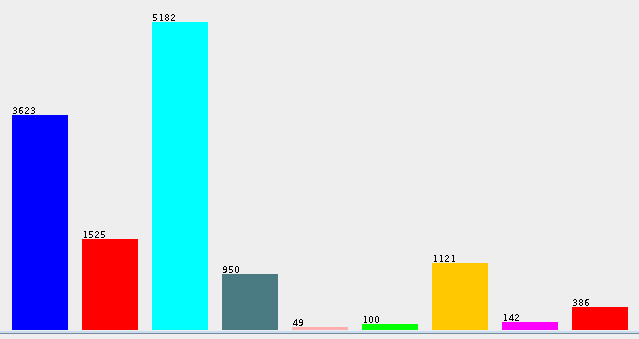
\includegraphics[width=0.8\textwidth]{images/attacktype.png}
  \caption{Distribution attack types}
  \label{fig:attack_distribution}
\end{minipage}
\begin{minipage}{0.49\textwidth}
  \centering
  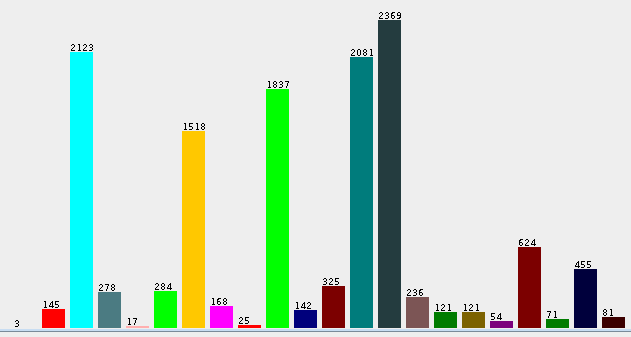
\includegraphics[width=0.8\textwidth]{images/victimtype.png}
  \caption{Distribution victim types}
  \label{fig:victim_distribution}
\end{minipage}
\end{figure}
The next limitation is that we do not take many features of terrorist organizations into account. We only have the features classification and geographical location into account. Now it is reasonable to think that there are other elements that maybe influence the decision of an attack or a victim type. One example is the average monthly income of a country. Maybe countries with a high average income carry out attacks that our much more sophisticated than in countries with a low average income. Due to time constraints we decided to only take the geographical location and classification into account. The results show that they weren't very good features unfortunately.\par
Another limitation of course was the amount of computation power we had. We only had a machine that could allocate 2,5 Gb for Weka. Like we already stated in section \ref{sec:apriori_3} this wasn't enough. There was also a server with 12 Gb but we couldn't really experiment on that because for every argument we changed we had to mail an executable to be ran on the server which would take a long time. That wasn't workable.
\section{What we also wanted to do}
We would really liked to have Apriori run on the third datafile, because the Apriori results were better than the J48 for the previous two datafiles. Also if we had more time we would have put the minimum support very low and let Apriori generate as much rules as possible. Than we can manually select the interesting rules for every attack type and victim type. We can determine the acceptable support for every possible type value manually.
\section{Conclusion}
\label{sec:conclusion}
In this document we tried to clearly explain what our plans were for the final homework, homework 6. We tried to structure this document according to the Crisp-DM model. It also contains which steps we already completed and which steps we still have to do.\par
Because this is a very elaborate and through explanation of what we have done already and are planning to do, it is very likely we will use parts of this document in the final report. As always all our code that we used can be found on our GitHub project\cite{githubproject}.
\printbibliography
\end{document}
